In chapter \ref{chap:unity}, the basic usage of Ubuntu was briefly touched upon. In this chapter, let's continue this trend and learn about how to install applications  in Ubuntu. Managing applications in Ubuntu is slightly different from its counterpart operating systems such as Windows and Mac OS. By the end of this chapter you will have know to how to install software, update and upgrade your system. In order to make this easy to grasp, where ever possible a reference or similarity to other operating systems will be mentioned.

\section{Ubuntu Software Center} \index{Ubuntu Software Center}
Contrary to installing applications in the Windows operating system where you need to scour the internet to find common applications like Firefox, Thunderbird or any other 3rd party application, in Ubuntu this can all be done right from your desktop using the Ubuntu Software Center which can be seen in figure \ref{fig:usc}. 

\begin{figure}[h!]	
	\centering
	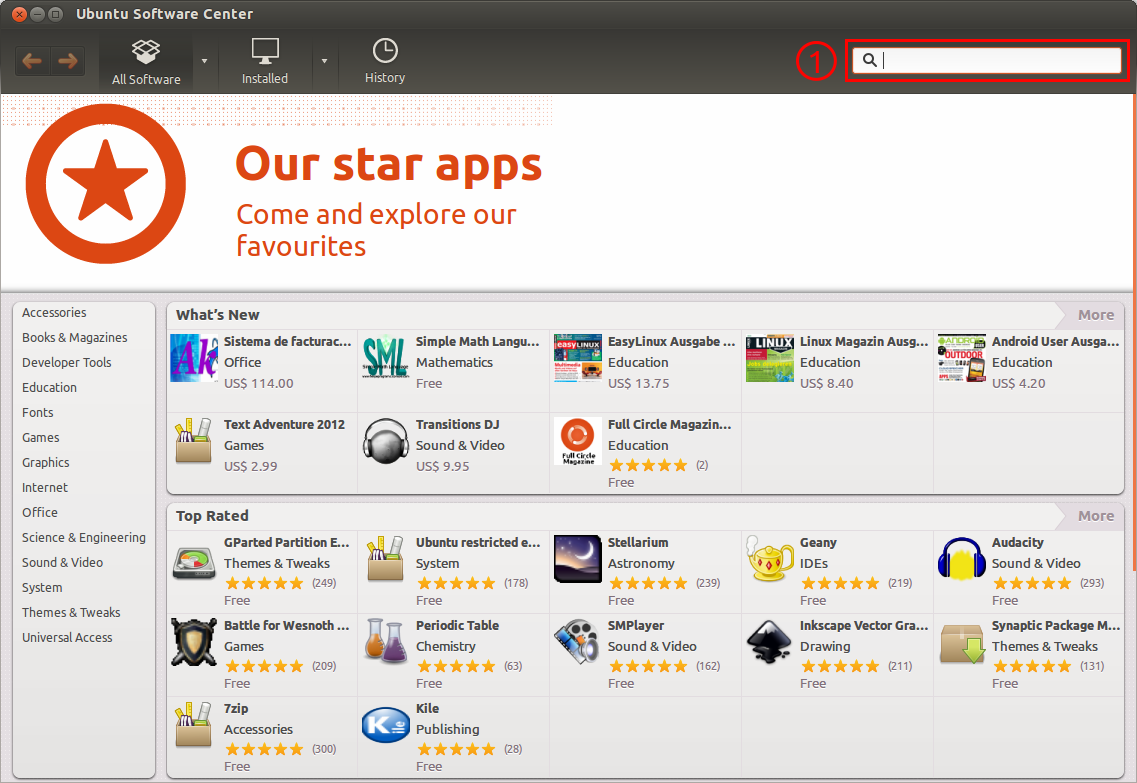
\includegraphics[width=325pt]{./images/applications/USC.png}
	\caption{Ubuntu Software Center}	
	\label{fig:usc}		
\end{figure}

\par \noindent You can launch the Ubuntu Software Center by pressing the Ubuntu Software Center icon in the launcher which looks like figure \ref{fig:usc-icon}. Or you can also launch Ubuntu Software Center from the dash as shown in section \ref{sect:dash}. 

\begin{figure}[h!]	
	\centering
	
\includegraphics[width=30pt]{./images/applications/usc-icon.png}
	\caption{Ubuntu Software Center launcher icon}	
	\label{fig:usc-icon}		
\end{figure}


\par \noindent The Ubuntu Software Center is a catalogue of applications, popular magazines and lenses. The Ubuntu Software Center is constantly being updated with new applications and content. If you are interested, you could yourself make an application which you submit for inclusion in the Ubuntu Software Center. It has a huge collection of applications produced by the community for the community. As can be seen in figure \ref{fig:usc}, the software center shows the top rated applications and also what's new. You can view applications by categories by clicking on one of the categories shown on the left. Try to explore the Ubuntu Software Center to get acquainted to the interface. It is a powerful application which can make managing application in Ubuntu much easier.\\

\section{Installing Application (via Ubuntu Software Center)} \label{sect:install-via-usc}

Let's try to install the program vlc using the software center.  You can do this by manually searching for vlc through the ``Sound and Video" category. However, a much quicker way is to search for vlc in the search box which can be in the top right of the software center (marked by a red box). On searching for vlc, you are presented with the search results as can be seen in figure \ref{fig:vlc-search}. 

\begin{figure}[h!]	
	\centering
	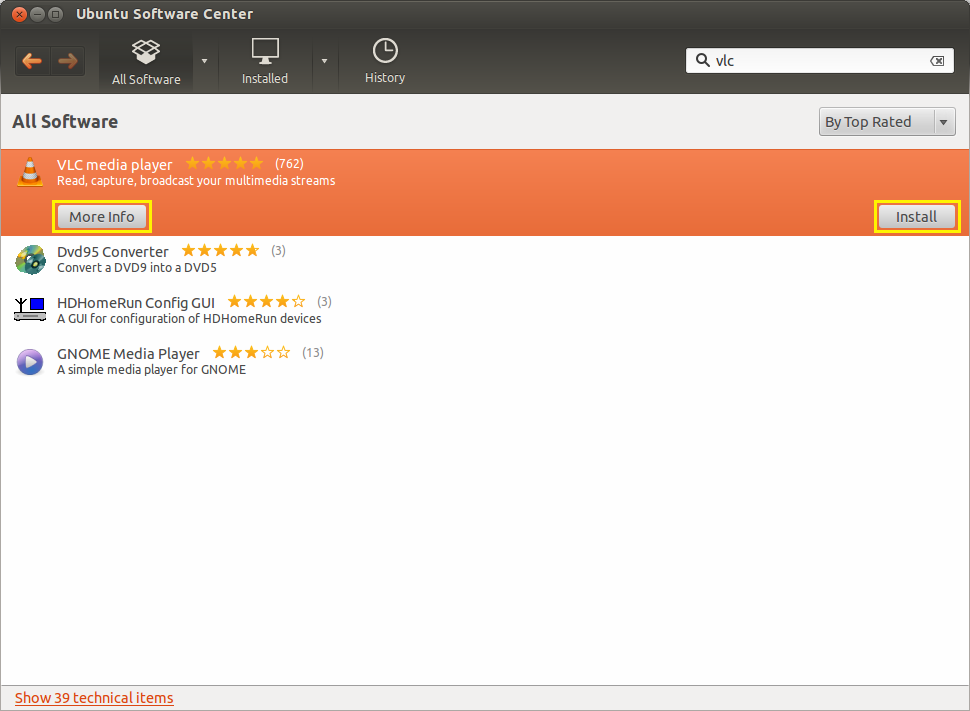
\includegraphics[width=300pt]{./images/applications/vlc-search.png}
	\caption{Search results}	
	\label{fig:vlc-search}		
\end{figure}

\par \noindent You can either install directly by pressing the install button. If you first wish to get more information about the application before you install, you can press more info. On pressing the more info button, you are presented with all the information about the application as seen in figure \ref{fig:vlc-info}. It shows the application description, the optional add-ons, reviews by other users and also other similar applications installed by other users.

\begin{figure}[h!]	
	\centering
	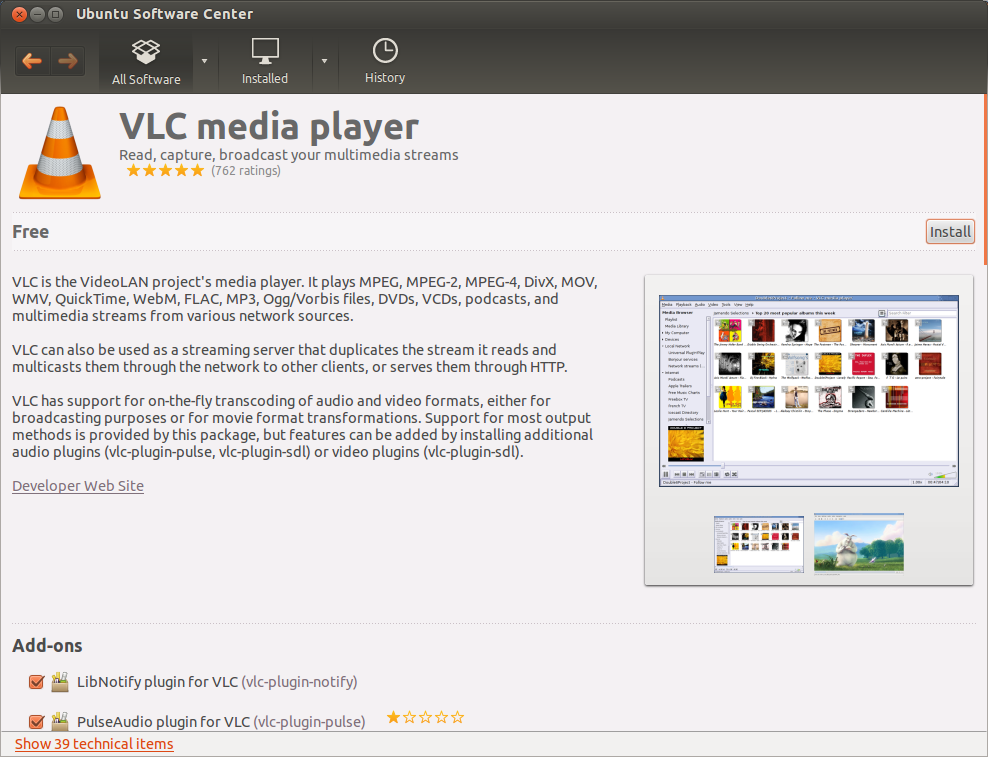
\includegraphics[width=300pt]{./images/applications/vlc-info.png}
	\caption{VLC application info}	
	\label{fig:vlc-info}		
\end{figure}

\par \noindent On pressing the install button, the installation starts in the background. You can either wait for it to install or you can do any other tasks that you wish to perform. You can keep a tab on the installation progress through the software center or in the launcher. This can be seen in figure \ref{fig:vlc-install}. \\

\begin{figure}[h!]	
	\centering
	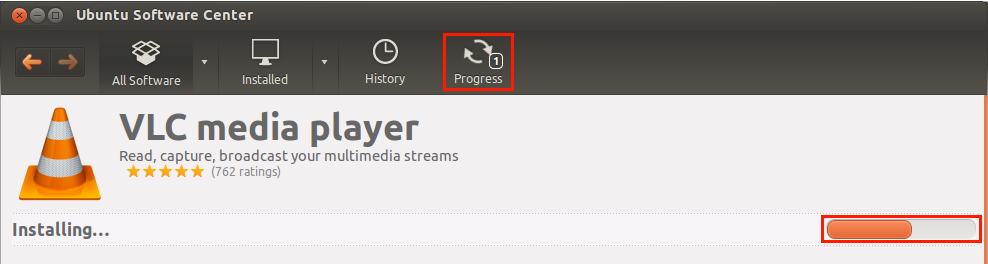
\includegraphics[width=325pt]{./images/applications/vlc-install.png}
	\caption{Installing vlc application}	
	\label{fig:vlc-install}		
\end{figure}

\par \noindent \framebox[6.7in][l]{\parbox[l]{6.5in}{\textbf{Tip}: You can install multiple applications at the same time without having to wait for one installation to complete to start another one. You can keep queuing applications you want to install. Ubuntu Software Center will automatically install all the queued applications one by one. }} \\

\section{Uninstalling Applications (via Ubuntu Software Center)}
As you saw in section \ref{sect:install-via-usc}, the installation process was a very simple task when done using the Ubuntu Software Center. Let's now see how to uninstall an application using the Ubuntu Software Center. The same application vlc will be used for this purpose. 

\begin{figure}[h!]	
	\centering
	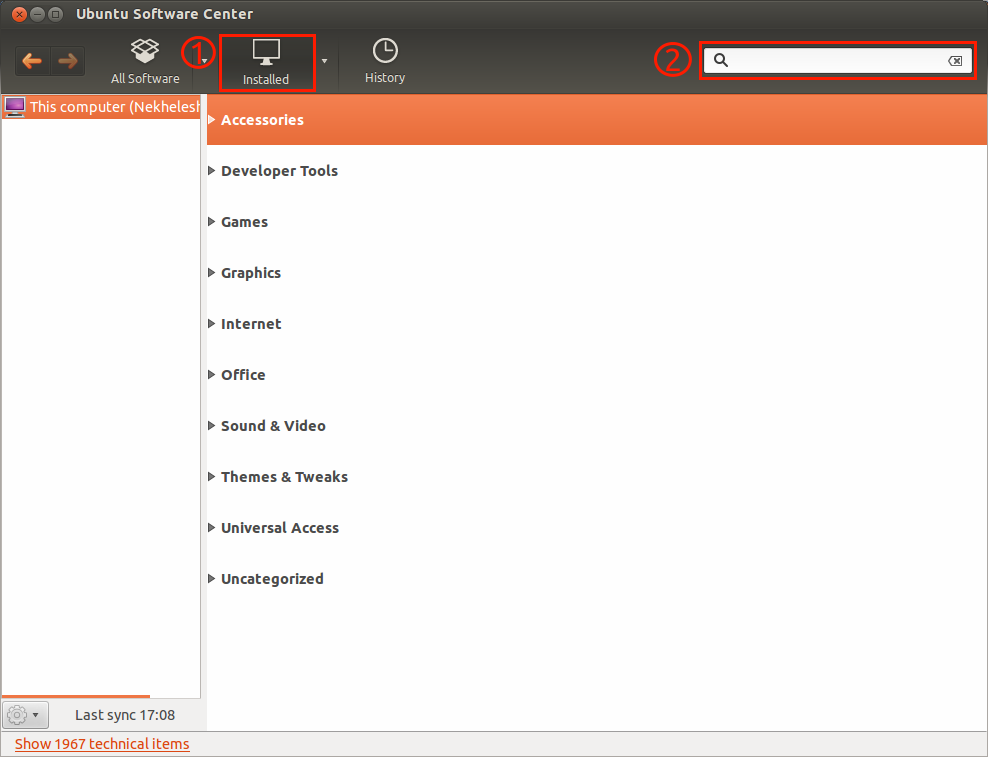
\includegraphics[width=325pt]{./images/applications/uninstall-apps.png}
	\caption{Uninstalling applications}	
	\label{fig:uninstall-apps}		
\end{figure}

\par \noindent First, you need to pressed the Installed button (marked with number 1) as can be seen in figure \ref{fig:uninstall-apps}. You are presented with the the different categories as seen in figure \ref{fig:uninstall-apps}. You can either search for vlc manually through the categories or you can search for vlc from search bar (marked by number 2) in figure \ref{fig:uninstall-apps}. When you search for vlc, the search results present vlc where you can uninstall by the clicking the button remove. This can be seen in figure \ref{fig:uninstall-vlc}.

\begin{figure}[h!]	
	\centering
	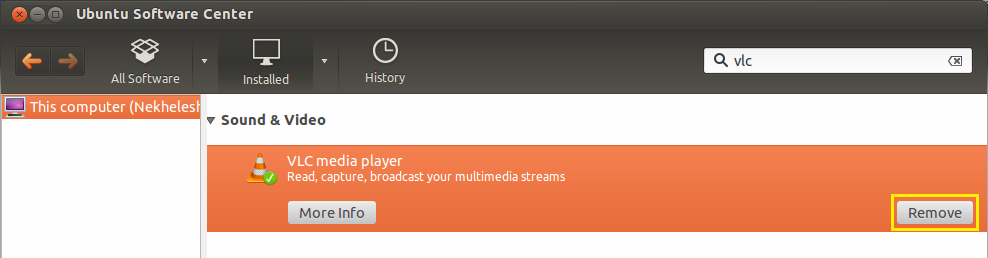
\includegraphics[width=325pt]{./images/applications/uninstall-vlc.png}
	\caption{Uninstalling vlc}	
	\label{fig:uninstall-vlc}		
\end{figure}

\section{Installation Applications (via other sources)}
Before proceeding further, it is important to explain a little bit about the application file type. In Windows, applications are distributed using executable files (.exe), while in Mac OS, you are given disk images (.dmg). In Ubuntu, applications are distributed in debian format (.deb). Remember this since you would be requiring this in the later part of this section. In the previous section, you were shown how to install applications using the Ubuntu Software Center. However, you are not constrained to installing application found in the Ubuntu Software Center. If you are unable to find your favourite application in the Ubuntu Software Center you can install that application using two other methods. \\

\par \noindent \framebox[6.7in][l]{\parbox[l]{6.5in}{\color{red} \textbf{Warning}: The installation methods described in this section allow the user to install other software, however please do not that installing software from random installation files (.deb) and Personal Package Package (PPA) found in the internet is not safe. They are not screened for security or stability. Use them with caution. All the softwares found in the Ubuntu Software Center has been carefully reviewed for these issues and is the best way to install applications in a secure manner.}} \\

\subsection*{Installation Files (.deb)} \index{deb}

The first method involves debian files (.deb). Let's illustrate this using an application such as Google Chrome. If you wanted to install Google Chrome, you can proceed to the Google's download page  \href{https://www.google.com/chrome}{\textit{here}}. Click download Google Chrome. You are then prompted with a dialog box asking which file you want to download as can be seen in figure \ref{fig:chrome-download}. Here you choose the 32-bit or 64-bit debian (.deb) file. This is marked by a red box in the figure.

\begin{figure}[h!]	
	\centering
	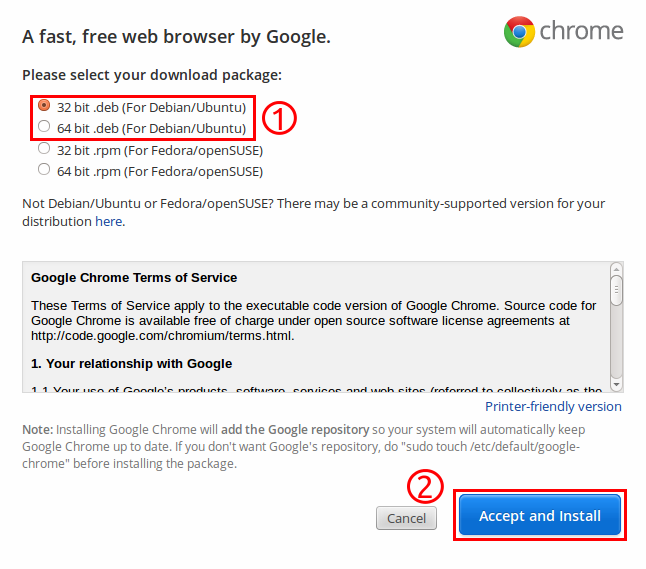
\includegraphics[width=300pt]{./images/applications/chrome-download.png}
	\caption{Download Google Chrome}	
	\label{fig:chrome-download}		
\end{figure}

\par \noindent Once it is downloaded to your system, you can find it in your Download folder by default. When you double click the installation file (.deb) as seen in figure \ref{fig:debfile-icon}, it is opened in the Ubuntu Software Center where you proceed to install it similar to the methods described in the previous sections. This disadvantage of installing applicating using .deb files is that these applications can only be updated manually and will not be done automatically using the update manager. \\

\begin{figure}[h!]	
	\centering
	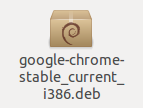
\includegraphics[width=60pt]{./images/applications/debfile-icon.png}
	\caption{Google Chrome Installation file (.deb)}	
	\label{fig:debfile-icon}		
\end{figure}

\par \noindent \framebox[6.7in][l]{\parbox[l]{6.5in}{\textbf{Note}: The Google Chrome .deb installation file is an exception to updates. The .deb file installs Google Chrome in your system and also configures a Personal Package Archive (PPA). This way Google Chrome is automatically updated when new versions are available due to the PPA. This is explained in more detail below.}} \\

\subsection*{Personal Package Archives (PPA)} \index{Personal Package Archive}

The second method to install applications is using Personal Package Archives (PPA). A Personal Package Archive can be thought of a personal database of applications. As long as you are connected to this database (PPA), you get updates and softwares whenever the database is updated. Let's take the example of Google Chrome explained before. Google has its own PPA or database where it keeps the latest version of Google Chrome. So when Google Chrome is installed on your system, it also connects your system to the PPA. This way if the PPA is updated with a new version of Google Chrome, you automatically receive it as an update thereby ensuring automation to keep the software up to date. \\ 

\par \noindent Most of the times it is necessary to manually connect your system to a PPA. This can be done by following the directions given below. Launch the Ubuntu Software Center from the dash or the launcher. In the software center, open the edit menu and click Software Sources. This is shown in figure \ref{fig:software-sources-menu}.

\begin{figure}[h!]	
	\centering
	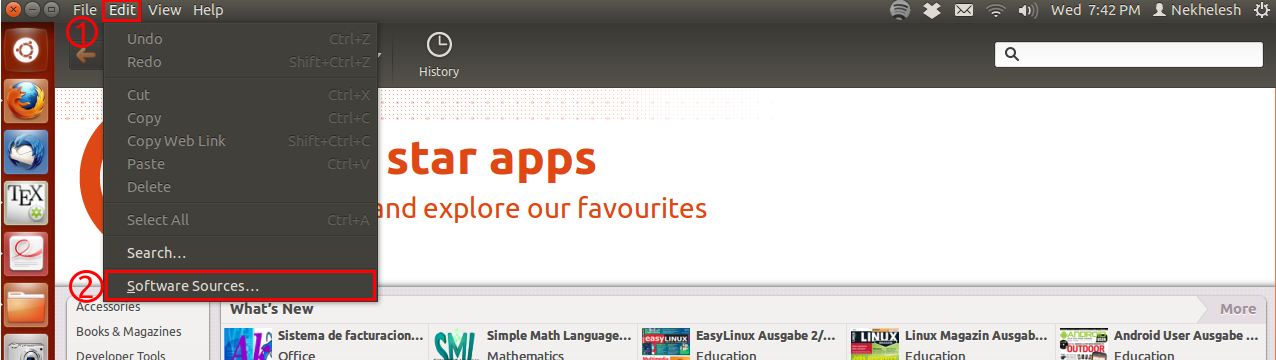
\includegraphics[width=350pt]{./images/applications/software-sources-menu.png}
	\caption{Software Sources Option}	
	\label{fig:software-sources-menu}		
\end{figure}

\par \noindent You are then presented with the software sources dialog as seen in figure \ref{fig:software-source}. Click on the Other Software tab.  \\

\begin{figure}[h!]	
	\centering
	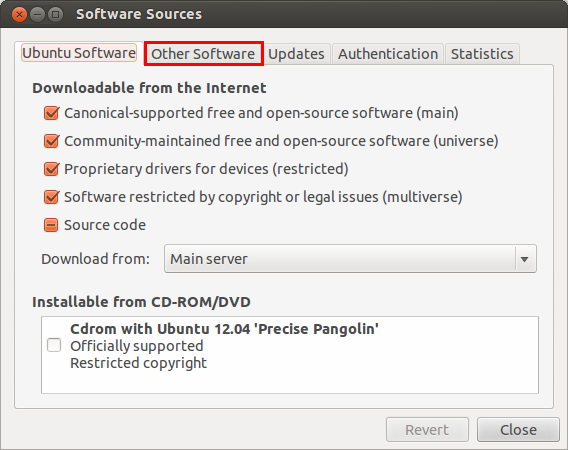
\includegraphics[width=300pt]{./images/applications/software-source.png}
	\caption{Software Sources Dialog}	
	\label{fig:software-source}		
\end{figure}

\par \noindent In the Other Software tab, you can see all the current PPA which are present in your system. In figure \ref{fig:software-source-ppa}, you can see the four launchpad PPA installed on this system.  \\

\begin{figure}[h!]	
	\centering
	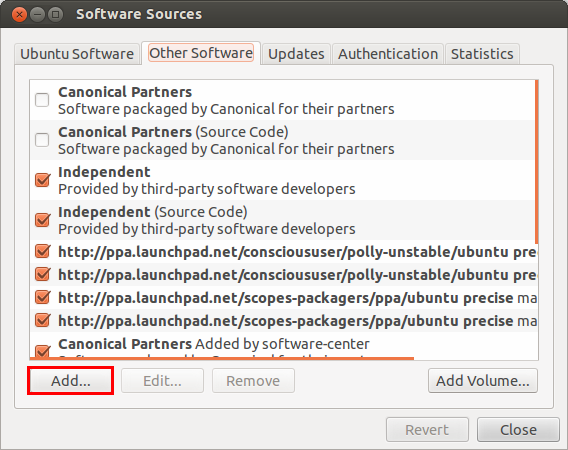
\includegraphics[width=300pt]{./images/applications/software-source-ppa.png}
	\caption{Software Sources - Other Software Tab}	
	\label{fig:software-source-ppa}		
\end{figure}

\par \noindent Click the Add button to add a PPA. In the Add PPA pop up dialog box as seen in figure x.xx, add the url to the PPA you want to install and click ok. You have now successfully added a PPA to your system. You need to now update the system manually using the update manager. You can launch the update manager from the dash. Click the check button in the update manager to check for updates manually. This is to inform the system about the newly added PPA. \\

\begin{figure}[h!]	
	\centering
	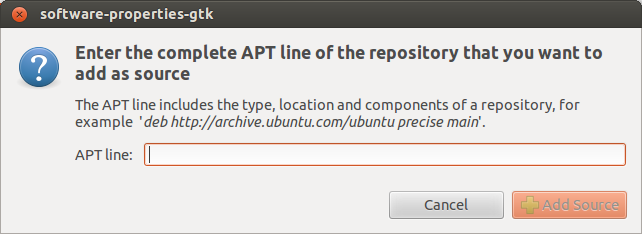
\includegraphics[width=300pt]{./images/applications/software-source-ppa-add.png}
	\caption{Software Sources - Add PPA}	
	\label{fig:software-source-ppa-add}		
\end{figure}

\par \noindent You can then install applications offered by the PPA directly from the software center. This is shown in figure \ref{fig:software-source-ppa-installapp}. In the figure \ref{fig:software-source-ppa-installapp}, you can see several PPA listed such as Polly Unstable PPA, Scopes Packagers Build, Tribler, Google etc. On selecting the PPA, you are then shown the list of application offered by that PPA. You can then proceed to install it similar to any other application.\\

\begin{figure}[h!]	
	\centering
	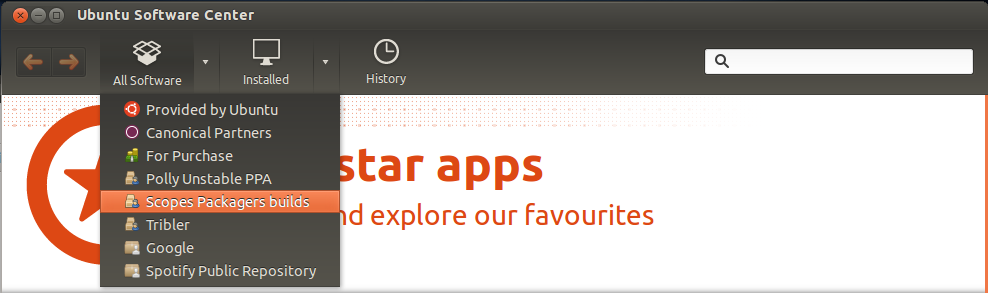
\includegraphics[width=350pt]{./images/applications/software-source-ppa-installapp.png}
	\caption{Software Sources - Install from PPA}	
	\label{fig:software-source-ppa-installapp}		
\end{figure}

\par \noindent \framebox[6.7in][l]{\parbox[l]{6.5in}{\textbf{Note}: Sometimes you might not see the PPA you recently added. This could be due to the software center not being refreshed yet. You can resolve this by restarting the software center or the system.}} \\

\section{Updates and Upgrades} \index{Updates} \index{Upgrades}
Just like other operating systems, it is important to update your Ubuntu system to ensure that your system is up to date and secure. Ubuntu will automatically prompt you for updates every week. The update manager will pop up showing the updates to all your software. The update manager can be seen in figure \ref{fig:update-manager}. If you want to check updates manually, you can do so by launching the update manager from the dash. There is however one important difference regarding updating in Ubuntu and other operating system. In Ubuntu, the update manager will show updates for all the applications installed in your system. This also includes the applications that you installed using the Ubuntu Software Center and using a Personal Package Archive (PPA). This is contrary to Windows, where the update manager only updates Windows and other Windows applications such as Microsoft Office etc. This way you do not need to worry about your installed applications being up to date. \\

\begin{figure}[h!]	
	\centering
	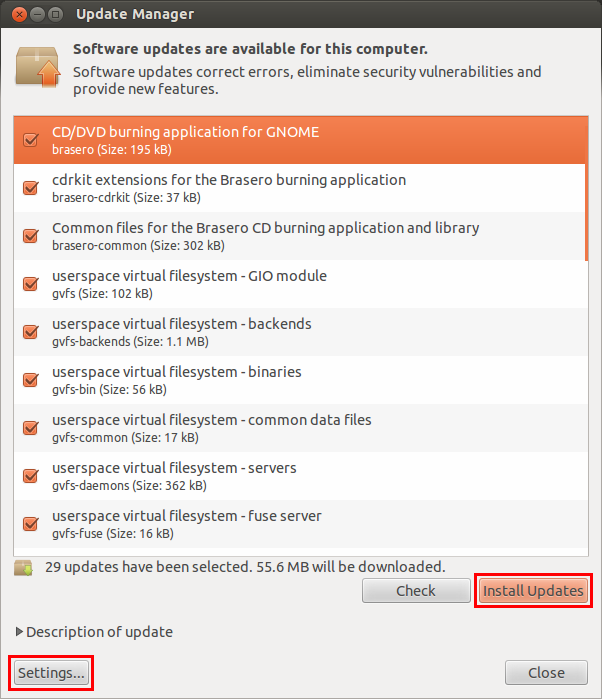
\includegraphics[width=325pt]{./images/applications/update-manager.png}
	\caption{Update manager}	
	\label{fig:update-manager}		
\end{figure}

\par \noindent It was explained in section \ref{chap:about_ubuntu_release} about new Ubuntu version released every 6 months while a new Long Term Support (LTS) is released every 2 years thought it is supported for 5 years on the desktop. You can choose to stick to the normal releases or stay with the LTS releases. You can change this setting by clicking on the settings button in the update manager as can be seen in figure \ref{fig:update-manager}. On clicking the button, you are presented with the settings dialog as can be seen in figure \ref{fig:update-preferences}. In the notify me of a new Ubuntu version, you can choose to be notified for new long term releases or for new normal releases. You will then be automatically prompted whenever a new version of Ubuntu is available. \\

\begin{figure}[h!]	
	\centering
	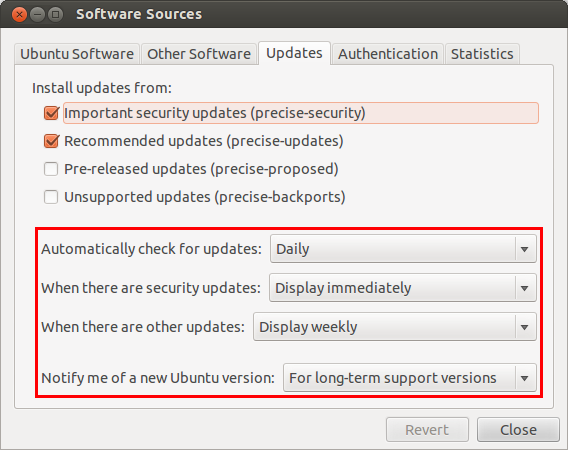
\includegraphics[width=325pt]{./images/applications/update-preferences.png}
	\caption{Update preferences}	
	\label{fig:update-preferences}		
\end{figure}

\par \noindent In the same settings dialog as seen in figure \ref{fig:update-preferences}, you can also set the frequency of the updates. By default, Ubuntu notifies of updates every week. You can change this to be displayed immediately or every two weeks.